\section{Data used for Validation}
\label{evaluation:data}

\subsection{Consumers}

This work considers real-world demand data of energy consumers.
It takes the data from two different sources.
\begin{enumerate*}[label=(\roman*)]
  \item Smart meters that Georgievski \citeauthor{Georgievski2012} installed in an office. \cite{Georgievski2012}
  \item Adaptive Charging Network (ACN) electric vehicle charging stations at the Californian Institute of Technology. \cite{Lee2019, ACNCaltech2020}
\end{enumerate*}

The data from the smart meters spans about $8$ months.
It is from the year 2016.
It has a time resolution of $10$ seconds.
The program transforms the data to have a time resolution of $10$ minutes.
It does so by adding up the energy demand of $10$ minute periods and then dividing by $0.166$ hours since the data is given as energy in kWh.
The result is the power given in kW.

The data from the ACN charging stations spans the first $9$ months of the year 2020.
It consists of various charging sessions.
The program identifies the energy demand by assuming the charger transfers energy to the car at one fixed rate in one session.
This is not the point of adaptive charging, but it gives a real-world-like representation of electric vehicle charging behavior.
The time resolution of the resulting data is $10$ minutes.

The program computes the average day of both datasets.
Then it combines both datasets.
The data from the smart meters is weighted $1, 000 : 1$ against the data from the ACN charging stations.
This composition is due to the low energy demand of one office.
The final data represents an average day of one electric vehicle charging site and $1, 000$ offices with a $10$ minute time resolution.
It is shown in figure \ref{figure:data.demand.day}.

\begin{figure}
  \centering
  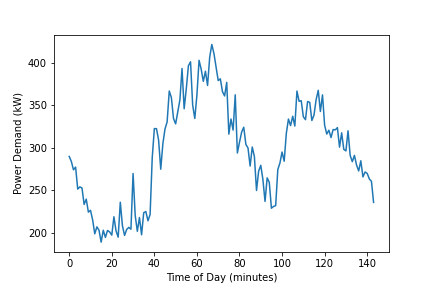
\includegraphics[width=0.7 \textwidth]{04_Validation/data_demand_day.png}
  \caption{Power Demand Data}
  \label{figure:data.demand.day}
\end{figure}

\subsection{Producers}

The data for the power plants is put together from different sources for different characteristics.
\begin{enumerate*}[label=(\roman*)]
  \item Maximum output power from a list by the \citeauthor{Kraftwerkliste2020}. \cite{Kraftwerkliste2020}
  \item Minimum power output from \cite{Schroder2013}.
  \item The startup and shutdown cost from \cite{Kumar2012}.
  \item Cost function coefficients from \cite{Alrashidi2009}.
\end{enumerate*}

From the list of german powerplants, $4$ plants are chosen, and their maximum output is taken.
All chosen plants are coal-powered power plants.
\cite{Kraftwerkliste2020}
$2$ of the plants are categorized as ''sub-critical'' and the other $2$ as ''super-critical''.
The difference between ''sub-critical'' and ''super-critical'' coal-powered power plants is the pressure level at which they operate.
''sub-critical'' power plants operate at pressure levels below $221$ bar and produce about $300$ to $900$ MW.
''super-critical'' power plants operate at pressure levels about $240$ bar and produce between $500$ to $1300$ MW.
\cite{Kumar2012, Schroder2013}
This choice is arbitrary but important for defining the other characteristics of the plants.

The minimum power output is computed based on the maximum power output and the type of power plant.
For ''sub-critical'' power plants, the minimal power output is $35\%$ of the maximum power output.
For ''super-critical'' power plants, the minimal power output is $20\%$ of the maximum power output.
\cite{Schroder2013}

The coal-powered power plants don't have shutdown costs.
So only the startup costs are computed.
For simplicity, this work only considers hot start startup costs.
For ''sub-critical'' power plants, the startup cost is $7.5$ MMBTU per MW maximum power output.
For ''super-critical'' power plants, the startup cost is $10.1$ MMBTU per MW maximum power output.
\cite{Kumar2012}
Where $1 \text{MMBTU} = 1.6 \cdot 10^{-6} \text{GJ}$.
This work considers all fuel costs in unit GJ.

The coefficients of the cost functions are taken from a paper that identified them at coal-powered power plants.
\cite{Alrashidi2009}
\citeauthor{Alrashidi2009} identified $2$ polynomials both are assigned randomly to the $4$ power plants.
The resulting values are presented in table \ref{table:evaluation.data.plants}.

\begin{table}[ht]
  \centering
  \begin{tabular}{| l || r | r | r | r |}
  \hline
  & Plant \#$1$ & Plant \#$2$ & Plant \#$3$ & Plant \#$4$ \\
  \hline \hline
  Maximum Power (MW) & $553$ & $747$ & $773$ & $1900$ \\ \hline
  Minimum Power (MW) & $193.55$ & $261.45$ & $145.6$ & $380$ \\ \hline
  Startup Cost (GJ) & $4.39635$ & $5.93865$ & $8.275738$ & $20.3414$ \\ \hline
  Constant Cost (GJ) & $95.856$ & $96.279$ & $95.856$ & $96.279$ \\ \hline
  Linear Cost $(\frac{\text{GJ}}{MW})$ & $7.374$ & $7.592$ & $7.374$ & $7.592$ \\ \hline
  Quadratic Cost $(\frac{\text{GJ}}{MW^2})$ & $0.047$ & $0.042$ & $0.047$ & $0.042$ \\ \hline
\end{tabular}
  \caption{Characteristics of Power Plants}
  \label{table:evaluation.data.plants}
\end{table}

\subsection{Model Sizes}

With the concrete values for the minimal and maximum power output of the power plants, the concrete size of the DQM and QUBO can be computed.
For this the formulas (\ref{formula:dqm.num.variables}), (\ref{formula:dqm.num.quadratic.biases}), (\ref{formula:qubo.num.variables}) and (\ref{formula:qubo.num.quadratic.biases}) are used.
The formulas give the size of the DQM and QUBO, respectively, based on the number of time instances, power plants, and the power output levels of the power plants.
They consider $2$ different metrics of the size:
\begin{enumerate*}[label=(\roman*)]
  \item The number of variables, which is the same as the number of linear biases ($v_{\text{DQM}}, v_{\text{QUBO}}$) and
  \item The number of quadratic biases ($q_{\text{DQM}}, q_{\text{QUBO}}$).
\end{enumerate*}

\subsubsection{Size of DQM}

For the DQM expanding the formulas (\ref{formula:dqm.num.variables}) and (\ref{formula:dqm.num.quadratic.biases}), and inserting the number of power plants is straight forward and gives the formulas (\ref{formula:dqm.num.variables.concrete}) and (\ref{formula:dqm.num.quadratic.biases.concrete}).
\begin{subequations}
\begin{align}
  \label{formula:dqm.num.variables.concrete}
  v_{\text{QUBO}} = & \aT \cdot \aI = 4 \cdot \aT \\
  \label{formula:dqm.num.quadratic.biases.concrete}
  q_{\text{QUBO}} = & \left( \aT - 1 \right) \cdot \aI + \aT \cdot \frac{\aI \cdot \left( \aI - 1 \right)}{2}
  = 4 \cdot \aT - 4 + 6 \cdot \aT = 10 \cdot \aT - 4
\end{align}
\end{subequations}

\subsubsection{Size of QUBO}

For the QUBO expanding the formulas (\ref{formula:qubo.num.variables}) and (\ref{formula:qubo.num.quadratic.biases}) is straight forward.
But we can not just insert the number of power plants into the formula.
We need to know how many power output levels each power plant has.
How the numbers are calculated is described in section \ref{approach:qubo.discretize}.
Table \ref{table:evaluation.data.plants.power.levels} shows the resulting numbers for the power output levels of the power plants.
\begin{table}[ht]
  \centering
  \begin{tabular}{| c | r | r |}
  \hline
  Power Plant $i$ & $n_i$ & $2^{n_i}$ \\
  \hline \hline
  0 & 6 & 64 \\
  \hline
  1 & 6 & 64 \\
  \hline
  2 & 7 & 128 \\
  \hline
  3 & 8 & 256 \\
  \hline
\end{tabular}
  \caption{Possible Power Output Levels of the Power Plants}
  \label{table:evaluation.data.plants.power.levels}
\end{table}

Inserting these values into the expanded formulas (\ref{formula:qubo.num.variables}) and (\ref{formula:qubo.num.quadratic.biases}) gives the formulas (\ref{formula:qubo.num.variables.concrete}) and (\ref{formula:qubo.num.quadratic.biases.concrete}).
\begin{subequations}
\begin{align}
\label{formula:qubo.num.variables.concrete}
  v_{\text{QUBO}} = & \aT \cdot \sum_{i \in \I} 2^{n_i} = \aT \cdot \left( 64 + 64 + 128 + 256 \right)
  = 1024 \cdot \aT
\\
\label{formula:qubo.num.quadratic.biases.concrete}
\begin{split}
  q_{\text{QUBO}} = & \left( \aT - 1 \right) \cdot 2 \cdot \sum_{i \in \I} 2^{n_i}
  + \aT \cdot \left(
    \sum_{i, j \in \I, i \neq j} 2^{n_i} \cdot 2^{n_j}
    + \sum_{i \in \I} \frac{2^{n_i} \cdot \left( 2^{n_i} - 1 \right)}{2}
  \right) \\
  = & \left( \aT - 1 \right) \cdot \left( 64 + 64 + 128 + 256 \right) \\
  & + \aT \left(
    2^{6 + 6} + 2^{6 + 7} \cdot 2 + 2^{6 + 8} \cdot 2 + 2^{7 + 8}
    + \frac{64 \cdot 63}{2} \cdot 2 + \frac{128 \cdot 127}{2} + \frac{256 \cdot 255}{2}
  \right) \\
  = & 130,816 \cdot \aT - 1,024
\end{split}
\end{align}
\end{subequations}
